\subsection{Lower-tail calibration in the critical window}\label{sec:calib}
Figure~\ref{fig:calib} compares the nominal lower-tail level with the actual lower-tail
probability in the failed test samples. The measured configurations have one-sided signs, lie
in the central window, and have failure probability at least about $0.03$. For these
configurations, when $M\ge256$ the additive corrections of selection and chi-square reduce the
grouped RMS relative error to about $0.04$--$0.08$; the unconditional threshold still carries
a substantial selection error.

The configurations included in each group differ across sizes, so the figure reports both the
dispersion and the number of configurations. The main theorem gives the direction and limiting
magnitude of the selection effect; this experiment gives the precision of the two analytic
corrections at finite size.
\begin{figure}[!htbp]
\centering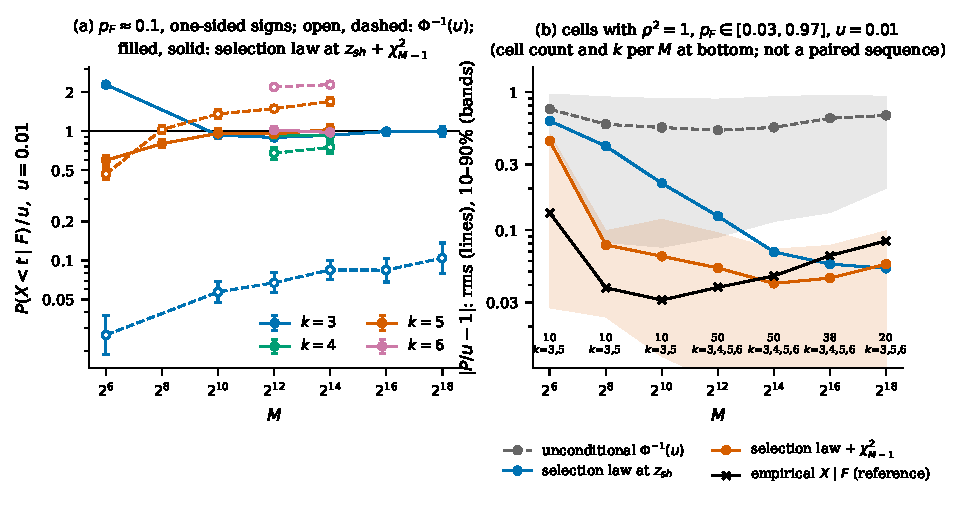
\includegraphics[width=\linewidth]{figures/fig_calib.pdf}
\caption{Lower-tail calibration in the central window. (a) ratio of the actual lower-tail
probability to its nominal value when the failure probability is about $0.1$ and all signs
positive; (b) root mean square relative error at the $\rho^2=1$ grid points.}
\label{fig:calib}
\end{figure}
